\documentclass{standalone}
\usepackage{pgfplots}
\pgfplotsset{compat=1.18}
\usepackage{tikz}
\usepackage{amsmath}
\usepackage{xcolor}
\usetikzlibrary{positioning, calc}

\definecolor{bb0Blue}{HTML}{1565c0}
\definecolor{bb1Green}{HTML}{2e7d32}
\definecolor{selfOrange}{HTML}{e65100}

\begin{document}
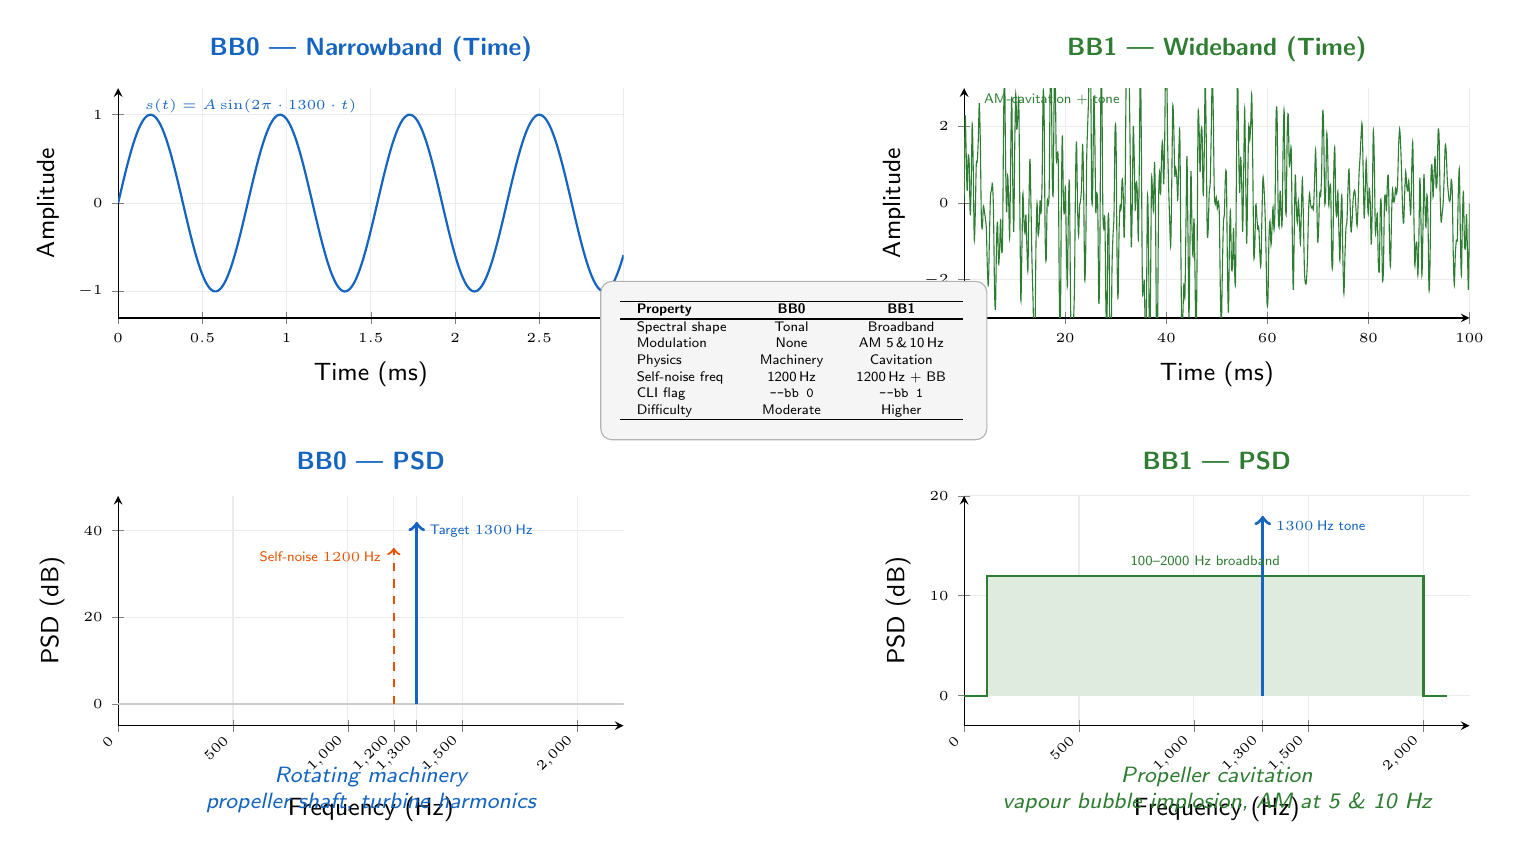
\begin{tikzpicture}[font=\sffamily\small]

%% ── BB0 Time domain ──────────────────────────────────────────────────────
\begin{axis}[
  name=bb0time,
  width=8cm, height=4.5cm,
  xmin=0, xmax=3, ymin=-1.3, ymax=1.3,
  title={\textbf{BB0 — Narrowband (Time)}},
  xlabel={Time (ms)}, ylabel={Amplitude},
  grid=both, grid style={black!8}, axis lines=left,
  title style={font=\sffamily\small, color=bb0Blue},
  tick label style={font=\sffamily\tiny}
]
  \addplot[bb0Blue, thick, smooth, samples=300, domain=0:3]
      {sin(deg(2*pi*1.3*x))};
  \node[bb0Blue, font=\sffamily\tiny, anchor=west] at (axis cs:0.1,1.1)
      {$s(t) = A\sin(2\pi\cdot1300\cdot t)$};
\end{axis}

%% ── BB0 PSD ──────────────────────────────────────────────────────────────
\begin{axis}[
  name=bb0psd,
  at={(bb0time.below south west)}, anchor=above north west, yshift=-0.6cm,
  width=8cm, height=4.5cm,
  xmin=0, xmax=2200, ymin=-5, ymax=48,
  title={\textbf{BB0 — PSD}},
  xlabel={Frequency (Hz)}, ylabel={PSD (dB)},
  grid=both, grid style={black!8}, axis lines=left,
  title style={font=\sffamily\small, color=bb0Blue},
  xtick={0,500,1000,1200,1300,1500,2000},
  xticklabel style={rotate=45, anchor=east, font=\sffamily\tiny},
  tick label style={font=\sffamily\tiny}
]
  \addplot[black!20, thin, domain=0:2200] {0};
  \addplot[bb0Blue, very thick, ->] coordinates {(1300,0)(1300,42)};
  \node[bb0Blue, anchor=west, font=\sffamily\tiny]
      at (axis cs:1315,40) {Target $1300\,\text{Hz}$};
  \addplot[selfOrange, dashed, thick, ->] coordinates {(1200,0)(1200,36)};
  \node[selfOrange, anchor=east, font=\sffamily\tiny]
      at (axis cs:1185,34) {Self-noise $1200\,\text{Hz}$};
\end{axis}

%% ── BB0 physics label ────────────────────────────────────────────────────
\node[bb0Blue, font=\sffamily\footnotesize\itshape,
      below=0.4cm of bb0psd.south, text width=7cm, align=center]
    {Rotating machinery\\propeller shaft, turbine harmonics};

%% ── BB1 Time domain ──────────────────────────────────────────────────────
\begin{axis}[
  name=bb1time,
  at={(bb0time.right of north east)}, anchor=left of north west, xshift=3.0cm,
  width=8cm, height=4.5cm,
  xmin=0, xmax=100, ymin=-3, ymax=3,
  title={\textbf{BB1 — Wideband (Time)}},
  xlabel={Time (ms)}, ylabel={Amplitude},
  grid=both, grid style={black!8}, axis lines=left,
  title style={font=\sffamily\small, color=bb1Green},
  tick label style={font=\sffamily\tiny}
]
  %% AM-modulated noise approximation
  \addplot[bb1Green, thin, smooth, samples=500, domain=0:100]
      {(1+0.5*sin(deg(2*pi*0.005*x))+0.5*sin(deg(2*pi*0.01*x)))*
       (0.9*sin(deg(2*pi*0.13*x))+0.7*sin(deg(2*pi*0.41*x))
       +0.8*sin(deg(2*pi*0.78*x))+0.6*sin(deg(2*pi*1.41*x)))
       +0.5*sin(deg(2*pi*1.3*x))};
  \node[bb1Green, font=\sffamily\tiny, anchor=west] at (axis cs:2,2.7)
      {AM-cavitation + tone};
\end{axis}

%% ── BB1 PSD ──────────────────────────────────────────────────────────────
\begin{axis}[
  name=bb1psd,
  at={(bb1time.below south west)}, anchor=above north west, yshift=-0.6cm,
  width=8cm, height=4.5cm,
  xmin=0, xmax=2200, ymin=-3, ymax=20,
  title={\textbf{BB1 — PSD}},
  xlabel={Frequency (Hz)}, ylabel={PSD (dB)},
  grid=both, grid style={black!8}, axis lines=left,
  title style={font=\sffamily\small, color=bb1Green},
  xtick={0,500,1000,1300,1500,2000},
  xticklabel style={rotate=45, anchor=east, font=\sffamily\tiny},
  tick label style={font=\sffamily\tiny}
]
  %% Broadband plateau 100-2000 Hz
  \addplot[bb1Green, thick, fill=bb1Green!15] coordinates
      {(0,0)(100,0)(100,12)(2000,12)(2000,0)(2100,0)};
  %% Tone spike
  \addplot[bb0Blue, very thick, ->] coordinates {(1300,0)(1300,18)};
  \node[bb0Blue, anchor=west, font=\sffamily\tiny]
      at (axis cs:1315,17) {$1300\,\text{Hz}$ tone};
  \node[bb1Green, font=\sffamily\tiny] at (axis cs:1050,13.5)
      {100--2000 Hz broadband};
\end{axis}

%% ── BB1 physics label ────────────────────────────────────────────────────
\node[bb1Green, font=\sffamily\footnotesize\itshape,
      below=0.4cm of bb1psd.south, text width=7cm, align=center]
    {Propeller cavitation\\vapour bubble implosion, AM at 5 \& 10 Hz};

%% ── Centre comparison table ─────────────────────────────────────────────
\node[draw=black!30, fill=black!4, rounded corners=4pt,
      font=\sffamily\tiny, inner sep=7pt, align=left]
      (tbl) at ($(bb0time.east)!0.5!(bb1time.west) + (0,-2.0)$) {
  \begin{tabular}{l c c}
    \hline
    \textbf{Property} & \textbf{BB0} & \textbf{BB1} \\\hline
    Spectral shape  & Tonal        & Broadband \\
    Modulation      & None         & AM 5\,\&\,10\,Hz \\
    Physics         & Machinery    & Cavitation \\
    Self-noise freq & 1200\,Hz     & 1200\,Hz + BB \\
    CLI flag        & \texttt{--bb 0} & \texttt{--bb 1} \\
    Difficulty      & Moderate     & Higher \\\hline
  \end{tabular}
};

\end{tikzpicture}
\end{document}
